\scalebox{0.8}{




\tikzset{every picture/.style={line width=0.75pt}} %set default line width to 0.75pt        

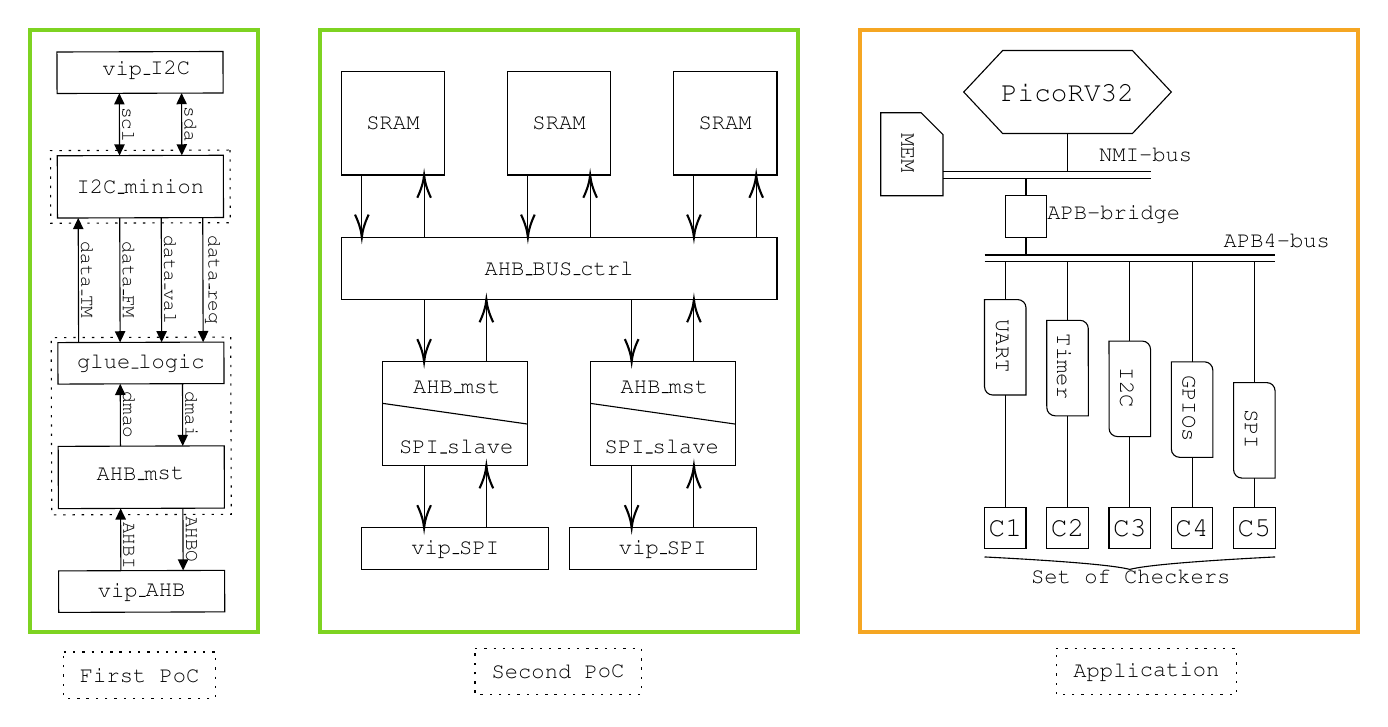
\begin{tikzpicture}[x=0.75pt,y=0.75pt,yscale=-1,xscale=1]
%uncomment if require: \path (0,335); %set diagram left start at 0, and has height of 335

%Shape: Rectangle [id:dp3731553954206104] 
\draw   (113.26,60.47) -- (113.35,90.47) -- (33.35,90.72) -- (33.26,60.72) -- cycle ;
%Shape: Rectangle [id:dp34474442632590674] 
\draw   (113.54,150.47) -- (113.6,170.47) -- (33.6,170.72) -- (33.54,150.72) -- cycle ;
%Shape: Rectangle [id:dp21177544535179416] 
\draw   (113.7,200.47) -- (113.79,230.47) -- (33.79,230.72) -- (33.7,200.72) -- cycle ;
%Shape: Rectangle [id:dp6089198540828209] 
\draw   (113.89,260.47) -- (113.95,280.47) -- (33.95,280.72) -- (33.89,260.72) -- cycle ;
%Shape: Rectangle [id:dp9980583574294419] 
\draw   (113.1,10.47) -- (113.16,30.47) -- (33.16,30.72) -- (33.1,10.72) -- cycle ;
%Shape: Rectangle [id:dp6022889606197361] 
\draw  [dash pattern={on 0.84pt off 2.51pt}] (116.5,57.96) -- (116.61,92.96) -- (30.11,93.23) -- (30,58.23) -- cycle ;
%Shape: Rectangle [id:dp5073417296194718] 
\draw  [dash pattern={on 0.84pt off 2.51pt}] (116.83,148.06) -- (117.1,233.46) -- (30.6,233.73) -- (30.33,148.33) -- cycle ;
%Straight Lines [id:da703665100005016] 
\draw    (93.17,33.53) -- (93.25,57.53) ;
\draw [shift={(93.26,60.53)}, rotate = 269.82] [fill={rgb, 255:red, 0; green, 0; blue, 0 }  ][line width=0.08]  [draw opacity=0] (5.36,-2.57) -- (0,0) -- (5.36,2.57) -- cycle    ;
\draw [shift={(93.16,30.53)}, rotate = 89.82] [fill={rgb, 255:red, 0; green, 0; blue, 0 }  ][line width=0.08]  [draw opacity=0] (5.36,-2.57) -- (0,0) -- (5.36,2.57) -- cycle    ;
%Straight Lines [id:da2788159188969581] 
\draw    (63.17,33.63) -- (63.25,57.63) ;
\draw [shift={(63.26,60.63)}, rotate = 269.82] [fill={rgb, 255:red, 0; green, 0; blue, 0 }  ][line width=0.08]  [draw opacity=0] (5.36,-2.57) -- (0,0) -- (5.36,2.57) -- cycle    ;
\draw [shift={(63.16,30.63)}, rotate = 89.82] [fill={rgb, 255:red, 0; green, 0; blue, 0 }  ][line width=0.08]  [draw opacity=0] (5.36,-2.57) -- (0,0) -- (5.36,2.57) -- cycle    ;
%Straight Lines [id:da06101786944370202] 
\draw    (103.35,90.5) -- (103.53,147.5) ;
\draw [shift={(103.54,150.5)}, rotate = 269.82] [fill={rgb, 255:red, 0; green, 0; blue, 0 }  ][line width=0.08]  [draw opacity=0] (5.36,-2.57) -- (0,0) -- (5.36,2.57) -- cycle    ;
%Straight Lines [id:da5424058149321302] 
\draw    (83.35,90.56) -- (83.49,135.56) -- (83.53,147.56) ;
\draw [shift={(83.54,150.56)}, rotate = 269.82] [fill={rgb, 255:red, 0; green, 0; blue, 0 }  ][line width=0.08]  [draw opacity=0] (5.36,-2.57) -- (0,0) -- (5.36,2.57) -- cycle    ;
%Straight Lines [id:da9873612100251858] 
\draw    (63.35,90.63) -- (63.53,147.62) ;
\draw [shift={(63.54,150.62)}, rotate = 269.82] [fill={rgb, 255:red, 0; green, 0; blue, 0 }  ][line width=0.08]  [draw opacity=0] (5.36,-2.57) -- (0,0) -- (5.36,2.57) -- cycle    ;
%Straight Lines [id:da17452981330250128] 
\draw    (43.36,93.69) -- (43.54,150.69) ;
\draw [shift={(43.35,90.69)}, rotate = 89.82] [fill={rgb, 255:red, 0; green, 0; blue, 0 }  ][line width=0.08]  [draw opacity=0] (5.36,-2.57) -- (0,0) -- (5.36,2.57) -- cycle    ;
%Straight Lines [id:da8963219174683734] 
\draw    (93.6,170.53) -- (93.69,197.53) ;
\draw [shift={(93.7,200.53)}, rotate = 269.82] [fill={rgb, 255:red, 0; green, 0; blue, 0 }  ][line width=0.08]  [draw opacity=0] (5.36,-2.57) -- (0,0) -- (5.36,2.57) -- cycle    ;
%Straight Lines [id:da9704047672943312] 
\draw    (63.61,173.62) -- (63.7,200.62) ;
\draw [shift={(63.6,170.62)}, rotate = 89.82] [fill={rgb, 255:red, 0; green, 0; blue, 0 }  ][line width=0.08]  [draw opacity=0] (5.36,-2.57) -- (0,0) -- (5.36,2.57) -- cycle    ;
%Straight Lines [id:da48527602904171707] 
\draw    (93.79,230.53) -- (93.88,257.53) ;
\draw [shift={(93.89,260.53)}, rotate = 269.82] [fill={rgb, 255:red, 0; green, 0; blue, 0 }  ][line width=0.08]  [draw opacity=0] (5.36,-2.57) -- (0,0) -- (5.36,2.57) -- cycle    ;
%Straight Lines [id:da8428632410120698] 
\draw    (63.8,233.62) -- (63.81,236.42) -- (63.89,260.62) ;
\draw [shift={(63.79,230.62)}, rotate = 89.82] [fill={rgb, 255:red, 0; green, 0; blue, 0 }  ][line width=0.08]  [draw opacity=0] (5.36,-2.57) -- (0,0) -- (5.36,2.57) -- cycle    ;
%Straight Lines [id:da7106944965440238] 
\draw    (460,68.5) -- (560,68.5)(460,71.5) -- (560,71.5) ;
%Straight Lines [id:da32567333179366464] 
\draw    (480,108.5) -- (620,108.5)(480,111.5) -- (620,111.5) ;
%Straight Lines [id:da5905899338537592] 
\draw    (500,72) -- (500,80) ;
%Shape: Rectangle [id:dp9222831914468617] 
\draw   (490,80) -- (510,80) -- (510,100) -- (490,100) -- cycle ;
%Straight Lines [id:da2570804632161796] 
\draw    (500,100) -- (500,108) ;
%Flowchart: Preparation [id:dp6591023232040161] 
\draw   (470,30) -- (488.75,10) -- (551.25,10) -- (570,30) -- (551.25,50) -- (488.75,50) -- cycle ;
%Snip Single Corner Rect [id:dp6798569296398] 
\draw   (430,40) -- (449.5,40) -- (460,50.5) -- (460,80) -- (430,80) -- cycle ;
%Straight Lines [id:da8928805450598687] 
\draw    (490,112) -- (490,130) ;
%Straight Lines [id:da615104418218078] 
\draw    (520,112) -- (520,140) ;
%Straight Lines [id:da6109908696043038] 
\draw    (550,112) -- (550,150) ;
%Straight Lines [id:da856254083187945] 
\draw    (580,112) -- (580,160) ;
%Straight Lines [id:da32215858489926874] 
\draw    (520,50) -- (520,68) ;
%Straight Lines [id:da42061995104894057] 
\draw    (520,120) -- (520,130) ;
%Rounded Diagonal Corner Rect [id:dp1323443763904859] 
\draw   (496,130) .. controls (498.21,130) and (500,131.79) .. (500,134) -- (500.01,176) .. controls (500.01,176) and (500.01,176) .. (500.01,176) -- (484.01,176) .. controls (481.8,176) and (480.01,174.21) .. (480.01,172) -- (480,130) .. controls (480,130) and (480,130) .. (480,130) -- cycle ;
%Rounded Diagonal Corner Rect [id:dp5665460653942873] 
\draw   (526,140) .. controls (528.21,140) and (530,141.79) .. (530,144) -- (530.01,186) .. controls (530.01,186) and (530.01,186) .. (530.01,186) -- (514.01,186) .. controls (511.8,186) and (510.01,184.21) .. (510.01,182) -- (510,140) .. controls (510,140) and (510,140) .. (510,140) -- cycle ;
%Rounded Diagonal Corner Rect [id:dp2172297870065225] 
\draw   (556,150) .. controls (558.21,150) and (560,151.79) .. (560,154) -- (560.01,196) .. controls (560.01,196) and (560.01,196) .. (560.01,196) -- (544.01,196) .. controls (541.8,196) and (540.01,194.21) .. (540.01,192) -- (540,150) .. controls (540,150) and (540,150) .. (540,150) -- cycle ;
%Rounded Diagonal Corner Rect [id:dp5688369530442512] 
\draw   (586,160) .. controls (588.21,160) and (590,161.79) .. (590,164) -- (590.01,206) .. controls (590.01,206) and (590.01,206) .. (590.01,206) -- (574.01,206) .. controls (571.8,206) and (570.01,204.21) .. (570.01,202) -- (570,160) .. controls (570,160) and (570,160) .. (570,160) -- cycle ;
%Straight Lines [id:da2564991599259481] 
\draw    (610,112) -- (610,170) ;
%Rounded Diagonal Corner Rect [id:dp6160675648140113] 
\draw   (616,170) .. controls (618.21,170) and (620,171.79) .. (620,174) -- (620.01,216) .. controls (620.01,216) and (620.01,216) .. (620.01,216) -- (604.01,216) .. controls (601.8,216) and (600.01,214.21) .. (600.01,212) -- (600,170) .. controls (600,170) and (600,170) .. (600,170) -- cycle ;
%Shape: Rectangle [id:dp0038058594335748097] 
\draw   (480,230) -- (500,230) -- (500,250) -- (480,250) -- cycle ;
%Shape: Rectangle [id:dp7339641035845104] 
\draw   (510,230) -- (530,230) -- (530,250) -- (510,250) -- cycle ;
%Shape: Rectangle [id:dp7389266519865625] 
\draw   (540,230) -- (560,230) -- (560,250) -- (540,250) -- cycle ;
%Shape: Rectangle [id:dp6929866930746469] 
\draw   (570,230) -- (590,230) -- (590,250) -- (570,250) -- cycle ;
%Shape: Rectangle [id:dp6258291809273131] 
\draw   (600,230) -- (620,230) -- (620,250) -- (600,250) -- cycle ;
%Straight Lines [id:da9888980297721972] 
\draw    (490,176) -- (490,230) ;
%Straight Lines [id:da3719517002576267] 
\draw    (520,186) -- (520,230) ;
%Straight Lines [id:da6253809938370463] 
\draw    (550,196) -- (550,230) ;
%Straight Lines [id:da8534944231471537] 
\draw    (580,206) -- (580,230) ;
%Straight Lines [id:da884643625523214] 
\draw    (610,216) -- (610,230) ;
\draw   (620,254) .. controls (581.11,256) and (557.78,258) .. (550,260) .. controls (542.22,258) and (518.89,256) .. (480,254) ;
%Shape: Square [id:dp8971117817457583] 
\draw   (170,20) -- (220,20) -- (220,70) -- (170,70) -- cycle ;
%Shape: Square [id:dp41424610009986873] 
\draw   (250,20) -- (300,20) -- (300,70) -- (250,70) -- cycle ;
%Shape: Square [id:dp6493258891670579] 
\draw   (330,20) -- (380,20) -- (380,70) -- (330,70) -- cycle ;
%Shape: Rectangle [id:dp8597198554400691] 
\draw   (190,160) -- (260,160) -- (260,210) -- (190,210) -- cycle ;
%Shape: Rectangle [id:dp5066171244331996] 
\draw   (170,100) -- (380,100) -- (380,130) -- (170,130) -- cycle ;
%Shape: Rectangle [id:dp37783869154825966] 
\draw   (290,160) -- (360,160) -- (360,210) -- (290,210) -- cycle ;
%Shape: Rectangle [id:dp7993038833874224] 
\draw   (180,240) -- (270,240) -- (270,260) -- (180,260) -- cycle ;
%Shape: Rectangle [id:dp7251500551853307] 
\draw   (280,240) -- (370,240) -- (370,260) -- (280,260) -- cycle ;
%Straight Lines [id:da37676367193377414] 
\draw    (190,180) -- (260,190) ;
%Straight Lines [id:da020888552157025897] 
\draw    (290,180) -- (360,190) ;
%Straight Lines [id:da8082119611875791] 
\draw    (180,70) -- (180,98) ;
\draw [shift={(180,100)}, rotate = 270] [color={rgb, 255:red, 0; green, 0; blue, 0 }  ][line width=0.75]    (10.93,-3.29) .. controls (6.95,-1.4) and (3.31,-0.3) .. (0,0) .. controls (3.31,0.3) and (6.95,1.4) .. (10.93,3.29)   ;
%Straight Lines [id:da2218971683921902] 
\draw    (210,100) -- (210,72) ;
\draw [shift={(210,70)}, rotate = 90] [color={rgb, 255:red, 0; green, 0; blue, 0 }  ][line width=0.75]    (10.93,-3.29) .. controls (6.95,-1.4) and (3.31,-0.3) .. (0,0) .. controls (3.31,0.3) and (6.95,1.4) .. (10.93,3.29)   ;
%Straight Lines [id:da8830096682726831] 
\draw    (290,100) -- (290,72) ;
\draw [shift={(290,70)}, rotate = 90] [color={rgb, 255:red, 0; green, 0; blue, 0 }  ][line width=0.75]    (10.93,-3.29) .. controls (6.95,-1.4) and (3.31,-0.3) .. (0,0) .. controls (3.31,0.3) and (6.95,1.4) .. (10.93,3.29)   ;
%Straight Lines [id:da02020197835555182] 
\draw    (370,100) -- (370,72) ;
\draw [shift={(370,70)}, rotate = 90] [color={rgb, 255:red, 0; green, 0; blue, 0 }  ][line width=0.75]    (10.93,-3.29) .. controls (6.95,-1.4) and (3.31,-0.3) .. (0,0) .. controls (3.31,0.3) and (6.95,1.4) .. (10.93,3.29)   ;
%Straight Lines [id:da12659652616674033] 
\draw    (260,70) -- (260,98) ;
\draw [shift={(260,100)}, rotate = 270] [color={rgb, 255:red, 0; green, 0; blue, 0 }  ][line width=0.75]    (10.93,-3.29) .. controls (6.95,-1.4) and (3.31,-0.3) .. (0,0) .. controls (3.31,0.3) and (6.95,1.4) .. (10.93,3.29)   ;
%Straight Lines [id:da07209741062271147] 
\draw    (340,70) -- (340,98) ;
\draw [shift={(340,100)}, rotate = 270] [color={rgb, 255:red, 0; green, 0; blue, 0 }  ][line width=0.75]    (10.93,-3.29) .. controls (6.95,-1.4) and (3.31,-0.3) .. (0,0) .. controls (3.31,0.3) and (6.95,1.4) .. (10.93,3.29)   ;
%Straight Lines [id:da3018302553747385] 
\draw    (210,130) -- (210,158) ;
\draw [shift={(210,160)}, rotate = 270] [color={rgb, 255:red, 0; green, 0; blue, 0 }  ][line width=0.75]    (10.93,-3.29) .. controls (6.95,-1.4) and (3.31,-0.3) .. (0,0) .. controls (3.31,0.3) and (6.95,1.4) .. (10.93,3.29)   ;
%Straight Lines [id:da8719656125359216] 
\draw    (310,130) -- (310,158) ;
\draw [shift={(310,160)}, rotate = 270] [color={rgb, 255:red, 0; green, 0; blue, 0 }  ][line width=0.75]    (10.93,-3.29) .. controls (6.95,-1.4) and (3.31,-0.3) .. (0,0) .. controls (3.31,0.3) and (6.95,1.4) .. (10.93,3.29)   ;
%Straight Lines [id:da6404760884518639] 
\draw    (240,160) -- (240,132) ;
\draw [shift={(240,130)}, rotate = 90] [color={rgb, 255:red, 0; green, 0; blue, 0 }  ][line width=0.75]    (10.93,-3.29) .. controls (6.95,-1.4) and (3.31,-0.3) .. (0,0) .. controls (3.31,0.3) and (6.95,1.4) .. (10.93,3.29)   ;
%Straight Lines [id:da6239987771072362] 
\draw    (340,160) -- (340,132) ;
\draw [shift={(340,130)}, rotate = 90] [color={rgb, 255:red, 0; green, 0; blue, 0 }  ][line width=0.75]    (10.93,-3.29) .. controls (6.95,-1.4) and (3.31,-0.3) .. (0,0) .. controls (3.31,0.3) and (6.95,1.4) .. (10.93,3.29)   ;
%Straight Lines [id:da48702991207504964] 
\draw    (210,210) -- (210,238) ;
\draw [shift={(210,240)}, rotate = 270] [color={rgb, 255:red, 0; green, 0; blue, 0 }  ][line width=0.75]    (10.93,-3.29) .. controls (6.95,-1.4) and (3.31,-0.3) .. (0,0) .. controls (3.31,0.3) and (6.95,1.4) .. (10.93,3.29)   ;
%Straight Lines [id:da39903471771483967] 
\draw    (240,240) -- (240,212) ;
\draw [shift={(240,210)}, rotate = 90] [color={rgb, 255:red, 0; green, 0; blue, 0 }  ][line width=0.75]    (10.93,-3.29) .. controls (6.95,-1.4) and (3.31,-0.3) .. (0,0) .. controls (3.31,0.3) and (6.95,1.4) .. (10.93,3.29)   ;
%Straight Lines [id:da7488758492286409] 
\draw    (310,210) -- (310,238) ;
\draw [shift={(310,240)}, rotate = 270] [color={rgb, 255:red, 0; green, 0; blue, 0 }  ][line width=0.75]    (10.93,-3.29) .. controls (6.95,-1.4) and (3.31,-0.3) .. (0,0) .. controls (3.31,0.3) and (6.95,1.4) .. (10.93,3.29)   ;
%Straight Lines [id:da21288565664023906] 
\draw    (340,240) -- (340,212) ;
\draw [shift={(340,210)}, rotate = 90] [color={rgb, 255:red, 0; green, 0; blue, 0 }  ][line width=0.75]    (10.93,-3.29) .. controls (6.95,-1.4) and (3.31,-0.3) .. (0,0) .. controls (3.31,0.3) and (6.95,1.4) .. (10.93,3.29)   ;
%Shape: Rectangle [id:dp37464523289284624] 
\draw  [color={rgb, 255:red, 126; green, 211; blue, 33 }  ,draw opacity=1 ][line width=1.5]  (20,0) -- (130,0) -- (130,290) -- (20,290) -- cycle ;
%Shape: Rectangle [id:dp0820690962764794] 
\draw  [color={rgb, 255:red, 126; green, 211; blue, 33 }  ,draw opacity=1 ][line width=1.5]  (160,0) -- (390,0) -- (390,290) -- (160,290) -- cycle ;
%Shape: Rectangle [id:dp432076382979272] 
\draw  [color={rgb, 255:red, 245; green, 166; blue, 35 }  ,draw opacity=1 ][line width=1.5]  (420,0) -- (660,0) -- (660,290) -- (420,290) -- cycle ;

% Text Node
\draw (76.13,19.08) node  [font=\footnotesize,rotate=-359.82] [align=left] {{\fontfamily{pcr}\selectfont vip\_I2C}};
% Text Node
\draw (73.3,75.59) node  [font=\footnotesize,rotate=-359.82] [align=left] {{\fontfamily{pcr}\selectfont I2C\_minion}};
% Text Node
\draw (73.57,160.59) node  [font=\footnotesize,rotate=-359.82] [align=left] {{\fontfamily{pcr}\selectfont glue\_logic}};
% Text Node
\draw (73.34,213.99) node  [font=\footnotesize,rotate=-359.82] [align=left] {{\fontfamily{pcr}\selectfont AHB\_mst}};
% Text Node
\draw (73.92,270.59) node  [font=\footnotesize,rotate=-359.82] [align=left] {{\fontfamily{pcr}\selectfont vip\_AHB}};
% Text Node
\draw (93.21,45.53) node [anchor=south] [inner sep=0.75pt]  [font=\scriptsize,rotate=-89.82] [align=left] {{\fontfamily{pcr}\selectfont sda}};
% Text Node
\draw (63.21,45.63) node [anchor=south] [inner sep=0.75pt]  [font=\scriptsize,rotate=-89.82] [align=left] {{\fontfamily{pcr}\selectfont scl}};
% Text Node
\draw (103.45,120.5) node [anchor=south] [inner sep=0.75pt]  [font=\scriptsize,rotate=-89.82] [align=left] {{\fontfamily{pcr}\selectfont data\_req}};
% Text Node
\draw (83.45,120.56) node [anchor=south] [inner sep=0.75pt]  [font=\scriptsize,rotate=-89.82] [align=left] {{\fontfamily{pcr}\selectfont data\_val}};
% Text Node
\draw (63.45,120.63) node [anchor=south] [inner sep=0.75pt]  [font=\scriptsize,rotate=-89.82] [align=left] {{\fontfamily{pcr}\selectfont data\_FM}};
% Text Node
\draw (43.45,120.69) node [anchor=south] [inner sep=0.75pt]  [font=\scriptsize,rotate=-89.82] [align=left] {{\fontfamily{pcr}\selectfont data\_TM}};
% Text Node
\draw (93.65,185.53) node [anchor=south] [inner sep=0.75pt]  [font=\scriptsize,rotate=-89.82] [align=left] {{\fontfamily{pcr}\selectfont dmai}};
% Text Node
\draw (63.65,185.62) node [anchor=south] [inner sep=0.75pt]  [font=\scriptsize,rotate=-89.82] [align=left] {{\fontfamily{pcr}\selectfont dmao}};
% Text Node
\draw (93.84,245.53) node [anchor=south] [inner sep=0.75pt]  [font=\scriptsize,rotate=-89.82] [align=left] {{\fontfamily{pcr}\selectfont AHBO}};
% Text Node
\draw (63.85,248.52) node [anchor=south] [inner sep=0.75pt]  [font=\scriptsize,rotate=-89.82] [align=left] {{\fontfamily{pcr}\selectfont AHBI}};
% Text Node
\draw (520,30) node   [align=left] {{\fontfamily{pcr}\selectfont PicoRV32}};
% Text Node
\draw (509,88.5) node [anchor=west] [inner sep=0.75pt]  [font=\footnotesize] [align=left] {{\fontfamily{pcr}\selectfont APB-bridge}};
% Text Node
\draw (443,59.5) node  [font=\footnotesize,rotate=-90] [align=left] {{\fontfamily{pcr}\selectfont MEM}};
% Text Node
\draw (488.5,152.5) node  [font=\footnotesize,rotate=-90] [align=left] {{\fontfamily{pcr}\selectfont UART}};
% Text Node
\draw (518.5,162.5) node  [font=\footnotesize,rotate=-90] [align=left] {{\fontfamily{pcr}\selectfont Timer}};
% Text Node
\draw (548.5,172.5) node  [font=\footnotesize,rotate=-90] [align=left] {{\fontfamily{pcr}\selectfont I2C}};
% Text Node
\draw (578.5,182.5) node  [font=\footnotesize,rotate=-90] [align=left] {{\fontfamily{pcr}\selectfont GPIOs}};
% Text Node
\draw (608.5,192.5) node  [font=\footnotesize,rotate=-90] [align=left] {{\fontfamily{pcr}\selectfont SPI}};
% Text Node
\draw (594,101.5) node [anchor=west] [inner sep=0.75pt]  [font=\footnotesize] [align=left] {{\fontfamily{pcr}\selectfont APB4-bus}};
% Text Node
\draw (534,60) node [anchor=west] [inner sep=0.75pt]  [font=\footnotesize] [align=left] {{\fontfamily{pcr}\selectfont NMI-bus}};
% Text Node
\draw (550.5,259) node [anchor=north] [inner sep=0.75pt]  [font=\footnotesize] [align=left] {{\fontfamily{pcr}\selectfont Set of Checkers}};
% Text Node
\draw (490,240) node   [align=left] {{\fontfamily{pcr}\selectfont C1}};
% Text Node
\draw (520,240) node   [align=left] {{\fontfamily{pcr}\selectfont C2}};
% Text Node
\draw (550,240) node   [align=left] {{\fontfamily{pcr}\selectfont C3}};
% Text Node
\draw (580,240) node   [align=left] {{\fontfamily{pcr}\selectfont C4}};
% Text Node
\draw (610,240) node   [align=left] {{\fontfamily{pcr}\selectfont C5}};
% Text Node
\draw (225,250) node  [font=\footnotesize,rotate=-359.82] [align=left] {{\fontfamily{pcr}\selectfont vip\_SPI}};
% Text Node
\draw (325,250) node  [font=\footnotesize,rotate=-359.82] [align=left] {{\fontfamily{pcr}\selectfont vip\_SPI}};
% Text Node
\draw (195,45) node  [font=\footnotesize,rotate=-359.82] [align=left] {{\fontfamily{pcr}\selectfont SRAM}};
% Text Node
\draw (275,45) node  [font=\footnotesize,rotate=-359.82] [align=left] {{\fontfamily{pcr}\selectfont SRAM}};
% Text Node
\draw (355,45) node  [font=\footnotesize,rotate=-359.82] [align=left] {{\fontfamily{pcr}\selectfont SRAM}};
% Text Node
\draw (275,115) node  [font=\footnotesize,rotate=-359.82] [align=left] {{\fontfamily{pcr}\selectfont AHB\_BUS\_ctrl}};
% Text Node
\draw (225.77,172.12) node  [font=\footnotesize,rotate=-359.82] [align=left] {{\fontfamily{pcr}\selectfont AHB\_mst}};
% Text Node
\draw (325.83,172.12) node  [font=\footnotesize,rotate=-359.82] [align=left] {{\fontfamily{pcr}\selectfont AHB\_mst}};
% Text Node
\draw (225.47,200.89) node  [font=\footnotesize,rotate=-359.82] [align=left] {{\fontfamily{pcr}\selectfont SPI\_slave}};
% Text Node
\draw (324.53,200.89) node  [font=\footnotesize,rotate=-359.82] [align=left] {{\fontfamily{pcr}\selectfont SPI\_slave}};
% Text Node
\draw  [dash pattern={on 0.84pt off 2.51pt}]  (36.44,299.81) -- (109.5,299.81) -- (109.5,322.02) -- (36.44,322.02) -- cycle  ;
\draw (72.97,310.92) node  [font=\footnotesize,rotate=-359.82] [align=left] {{\fontfamily{pcr}\selectfont First PoC}};
% Text Node
\draw  [dash pattern={on 0.84pt off 2.51pt}]  (234.5,297.99) -- (314.56,297.99) -- (314.56,320.23) -- (234.5,320.23) -- cycle  ;
\draw (274.53,309.11) node  [font=\footnotesize,rotate=-359.82] [align=left] {{\fontfamily{pcr}\selectfont Second PoC}};
% Text Node
\draw  [dash pattern={on 0.84pt off 2.51pt}]  (514.5,297.99) -- (601.56,297.99) -- (601.56,320.25) -- (514.5,320.25) -- cycle  ;
\draw (558.03,309.12) node  [font=\footnotesize,rotate=-359.82] [align=left] {{\fontfamily{pcr}\selectfont Application}};


\end{tikzpicture}
}
